\section{Comércio Eletrônico}


\subsection{\textit{E-Commerce Security}} \label{e-commerce-secutiry}

Comércio eletrônico (\textit{E-Commerce}\nomenclature{E-Commerce}{Comércio Eletrônico}) é a compra e venda de mercadorias pela Internet. Atividades comerciais na Internet tem crescido exponecialmente nos últimos anos \cite{al2008commerce}. No atual mercado globalizado, qualquer negócio, para ser competitivo, necessita de políticas de segurança abrangentes, em conformidade com seus parceiros, para prover ambientes seguros para a realização de atividades de comércio eletrônico \cite{al2008commerce}.

Para prover tais ambientes seguros, uma Infra Estrutura de Chaves Públicas - ICP\nomenclature{ICP}{Infra Estrutura de Chaves Públicas} (\textit{Public Key Infrastructure}, PKI\nomenclature{PKI}{\textit{Public Key Infrastructure}}) pode ser utilizada para estabelecer comunicações seguras em uma rede, utilizando criptografia de chaves públicas. ICP define um ambiente onde usuários podem trasmitir certificados que os identificam \cite{al2008commerce}. 

Aplicações de \textit{E-Commerce} também podem funcionar \textit{Secure Electronic Transfer} (SET)\nomenclature{SET}{\textit{Secure Electronic Transfer}} ou \textit{Secure Socket Layer} (SSL)\nomenclature{SSL}{\textit{Secure Socket Layer}} para criptografia de tranmissões de dados utilizando os protocolos TCP/IP \cite{al2008commerce}.

No ciberespaço, tanto clientes quanto vendedores tem dificuldades em prover sua identifidade um para o outro com certeza, particularmente durante a primeira transação. Algumas questões levantadas em \cite{al2008commerce}, apresentadas a seguir, descrevem problemas que afetam transações comerciais em uma rede de computadores pública, como a Internet: Como o comprador transmite informações sensíveis para o vendedor? Como o vendedor conhece uma ordem de compra legítima? Como ambas as partes sabem que um terceiro mal intecionado não copiou ou alterou as informações da transação? 

\cite{al2008commerce} indica que clientes precisam garantir que:
\begin{itemize}
	\item eles estão se comunicando com o servidor correto;
  \item o que eles enviam é entregue sem modificações;
  \item eles podem provar que enviaram a mensagem;
  \item somente o destinatário desejado pode ler a mensagem; e
  \item a entrega é garantida.
\end{itemize}

No lado dos vendedores, eles precisam ter garantia que \cite{al2008commerce}:

\begin{itemize}
	\item eles estão se comunicando com o cliente correto;
	\item o conteúdo da mensagem recebida está correto;
	\item a identidade do autor não pode ser falsificada;
	\item somente o autor declarado pode realmente ter escrito a mensagem; e
	\item eles confirmam o recebimento da mensagem.
\end{itemize}

Em \cite{jiang2007line} são citados alguns fatores de segurança que aplicações de \textit{E-Commerce} devem considerar, como: confidencialidade, integridade, validade e não repúdio da informação e autenticidade.

Ambas as partes também não podem repudiar uma mensagem que enviaram \cite{jiang2007line}, por exemplo, um cliente legítimo que realizou um pedido de compra não tem como negar que o fez. O receptor deve ter como confirmar que a mensagem recebida é realmente do emissor informado na mensagem, e o emissor deve ter garantia de que somente o destinatário designado poderá ler a mesma \cite{jiang2007line}. São necessários mecanismos para identificar a integridade das informações trocadas, para saber quando as mesmas foram alteradas \cite{jiang2007line}, intecionalmente, devido a ação de \textit{crackers} ou não, devido a falhas de hardware e software.

Todos as preocupações listadas acima podem ser resolvidas usando alguma combinação de métodos criptográficos e métodos de certificado. Os tipos de risco resultante de inadequada segurança, segundo \cite{al2008commerce}, são:

\begin{itemize}
	\item bugs ou problemas de configurações incorretas no servidor Web, que podem causar roubo de documentos confidenciais;
	\item brechas de segurança no lado do cliente, que podem comprometer sua privacidade e danificar seu sistema;
	\item interceptação de dados enviados do cliente para o servidor, e vice-versa. Isto é possível em qualquer parte do caminho entre a rede do cliente e a o servidor, na rede do provedor de Internet do usuário ou outros provedores regionais.
\end{itemize}

\subsubsection{Políticas de Medidas de Segurança em \textit{E-Commerce}}

Segundo \cite{al2008commerce}, existem três diferentes políticas usadas para garantir e medir a segurança em ambientes de \textit{E-Commerce}, que são: privacidade, criptografia e certificados.

%\subsubsection{Política de Privacidade}
\textbf{Política de Privacidade}

Política de Privacidade são utilizadas para arquitetar a forma em que uma companhia coleta, usa, protege dados es escolhas que eles oferecem aos consumidores quando suas informações pessoais são utilizadas. Baseados nessa política, consumidores podem determinar se e com qual extensão eles desejam disponibilizar informações para a companhia.

%\subsubsection{Criptografia}
\textbf{Criptografia}

Sistemas de cifragem (criptografia) são classificados em duas classes, apresentadas a seguir.


\textbf{Sistemas de Chave Secreta}

A criptografia de chave secreta é o mais antigo método criptográfico, tendo dois principais tipos: a cifragem por transporte e por substituição. O primeiro criptografa a mensagem original alterando a ordem dos caracteres. O segundo substitui os caracteres da mensagem por outros. Em ambos os casos, o emissor e o receptor compartilham a mesma chave secreta. O algoritmo de chave secreta mais amplamente utilizado atualmente é o \textit{Data Encryptation Standard} (DES)\nomenclature{DES}{\textit{Data Encryptation Standard}}, que funciona com uma chave secreta de 56 bits e 16 iterações para transformar um bloco de texto plano em texto cifrado.

\textbf{Sistemas de Chave Pública}

A criptografai de chave pública foi desenvolvida para resolver o problema de distribuição de chaves secretas. O primeiro algoritmo foi publicamente descrito em 1976 pelo professor Martin Hellman, da Universidade de Stanford, e seu aluno graduando Whitfield Diffie. Tais métodos utilizam duas diferentes chaves matematicamente relacionadas. Uma chave é usada para criptografar os dados, e a segunda para descriptografar. O segundo problema que Diffie ponderou foi o de "assinaturas digitais". O esquema de Rivest Shamir-Adleman (RSA) é o mais conhecidamente aceito e implementado algoritmo de propósito geral para criptografia de chave pública. O esquema é uma cifra de bloco em que o texto plano e o texto cifrado são inteiros entre 0 e n-1 for algum n. Um tamanho típico para n é 1024 bits, ou 309 dígitos decimais. O tamanho de bloco deve ser menor ou igual a log2(n). Segundo \cite{al2008commerce}, a criptografia e a descriptografia são da seguinte forma, para algum texto plano M e um texto cifrado C:
\begin{center}
	\begin{equation}
		C=M^e\:mod\:n%\: incluir espaço entre elementos da equação
	\end{equation}
	\captionof{equation}{Cifragem com RSA \cite{al2008commerce}}
	\label{eq:rsa-cifragem}
\end{center}

\begin{center}
	\begin{equation}
    %\: incluir espaço entre elementos da equação
		M \: = \: C^d \: mod \: n \: = \: (M^e)^d \: mod \: n \: = \: M^{ed} \: mod \: n 
	\end{equation}
	\captionof{equation}{Decifragem com RSA \cite{al2008commerce}} 
	\label{eq:rsa-decifragem}
\end{center}

Ambos emissor e receptor devem conhecer o valor de \textit{n}. O emissor conhece o valor de \textit{e}, e somente o receptor conhece o valor de \textit{d}. Assim, segundo \cite{al2008commerce}, este é um algoritmo de chave pública com:
\begin{itemize}
	\item uma chave pública de $ KU=\{e,n\} $
	\item uma chave privada de $ KR=\{d,n\} $
\end{itemize}

%\subsubsection{Certificado}
\textbf{Certificado}

Certificados associam identidade, autoridade, chave pública e outras informações do usuário. Para a maioria das aplicações de \textit{E-Commerce}, certificados usam um formato definido pelo \textit{International Telecommunication Union - Telecomunication Standardization Sector} (ITU-T)\nomenclature{ITU-T}{\textit{International Telecommunication Union - Telecomunication Standardization Sector}}, tal como a recomendação X.509. Segundo \cite{al2008commerce}, certificados X.509 contêm informações como:
\begin{itemize}
	\item nome, identificação e chave pública do proprietário do certificado;
	\item nome e identificação do emissor do certificado; 
	\item definições de limitações de uso, informações de políticas e período de validade do certificado.
\end{itemize}

Com uso de certificados digitais, compradores podem obter um certificado digital pessoal para provar sua identidade para um Web \textit{site}, mas os vendedores é que realmente precisam de certificados para provar sua identidade para os compradores.

\subsubsection{\textit{Pretty Good Privacy} (PGP)}\nomenclature{PGP}{\textit{Pretty Good Privacy}}

PGP provê um serviço de autenticação e confidencialidade que pode ser usado para \textit{e-mail} e aplicações de armazenamento de arquivos. Ele tem crescido explisivamente e é amplamente utilizado na atualidade. Segundo \cite{al2008commerce}, três razões podem ser citadas para isto:

\begin{itemize}
	\item ele é baseado em algoritmos que tem sobrevivido a extensas revisões públicas e são considerados extremamente seguros;
	\item ele tem uma ampla faixa de aplicabilidade;
	\item ele não foi desenvolvido nem é controlado por qualquer órganização governamental ou de padronização.
\end{itemize}

A atual operação do PHP consiste de cinco serviços: autenticação, confidencialidade, compressão, compatibilidade de e-mail e segmentação. A seguir são examinados os dois primeiros serviços, que podem ser utilizados para \textit{E-Commerce}.

%\subsubsection{Autenticação}
\textbf{Autenticação}

Transações na Internet são realizadas entre computadores geograficamente distantes. Desta forma as partes precisam reconhecer e confiar uma na outra \cite{jiang2007line}, especialmente em trasações de \textit{E-Commerce}, por envolverem dinheiro. Para isso, são necessários mecanismos de autenticação das partes.

Autenticação requer uma assinatura digital. O processo inicia com um resumo matemático denominado \textit{hash}, que age como uma impressão digital da mensagem. Assim, se a mensagem for alterada, se tornará incompatível com o \textit{hash} original. Este código \textit{hash} é criptografado com a chave primava do remetente e anexado à mensagem. Quando a mensagem é recebida, o código \textit{hash}, anexado a ela, é comparado com outro código \textit{hash} calculado pelo receptor. Chaves para assinaturas digitais são armazenadas em um diretório de chaves públicas, composto de "certificados" para todos os usuários. \cite{al2008commerce} Uma Autoridade Certificadora confiável gerencia e distribui estes certificados, para permitir a distribuição de chaves eletrônicas. O esquema de assinatura digital é apresentado na sequência abaixo e na Figura \ref{fig:pgp-authentication}.

\begin{itemize}
\item Geração de mensagem e assinatura pelo emissor:
	\begin{itemize}
		\item o emissor cria uma mensagem;
		\item algoritmo de \textit{hash} SHA-1 é usado para gerar um código \textit{hash} de 160 bits da mensagem;
		\item o código \textit{hash} é criptografado com RSA, usando a chave privada do emissor, e o resultado é acrescentado à mensagem.
    {\color{red}Este \textit{hash} criptografado é a assinatura digital da mensagem.} 
	\end{itemize}

\item Verificação da autenticidade da mensagem pelo receptor:
	\begin{itemize}
		\item o receptor usa RSA com a chave pública do emissor para descriptografar e recuperar o \textit{hash};
		\item o receptor gera um novo \textit{hash} a partir da mensagem, usando a chave pública do emissor e {\color{red}RSA},
    e compara este \textit{hash} com o \textit{hash} recebido e descriptografado. 
    Se os dois correspondem, a mensagem é aceita como autêntica.
	\end{itemize}
\end{itemize}

\begin{center}
	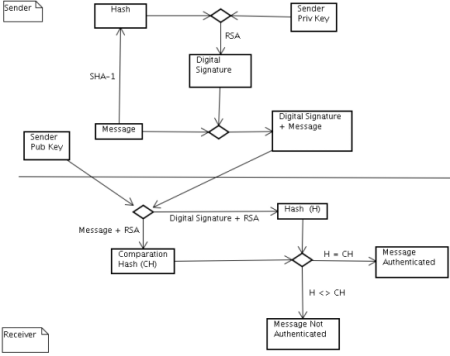
\includegraphics[scale=0.8]{images/pgp-authentication.png}
	\captionof{figure}{Autenticação em PGP}
	\label{fig:pgp-authentication}
\end{center}

A combinação de SHA-1 e RSA provê um efetivo esquema de assinatura digital. Devido à força do RSA, o receptor tem garantia de que somente o possuidor da chave privada pôde ter gerado a assinatura; e devido à força do SHA-1, ele tem garantia de que ninguém pode gerar uma mensagem que corresponda com o código \textit{hash} e com a assinatura da mensagem original. Embora assinaturas normalmente são anexadas à mensagem ou arquivo que elas assinam, assinaturas não anexadas também são suportadas. Estas podem ser armazenadas e transmitidas separadamente da mensagem que elas assinam.

%\subsubsection{Confidencialidade}
\textbf{Confidencialidade}

O emissor e receptor de uma mensagem precisam garantir a confidencialidade na troca de informações, principalmente em um ambiente de \textit{E-Commerce}. Assim, para previnir transações neste ambiente de roubo de informações, é preciso garantir que apenas usuários legítimos serão capazes de ver os dados\cite{jiang2007line}.

Confidencialidade é provida pela criptografia da mensagem a ser transmitida ou a ser armazenada localmente. O esquema é apresentado na sequência abaixo e na Figura \ref{fig:pgp-confidentiality}.

\begin{itemize}
  \item Geração de mensagem criptografada a ser aberta somente por um determinado destinatário
	\begin{itemize}
		\item o emissor gera uma mensagem e um número aleatório de 128 bits para ser usada como uma chave de sessão somente para esta mensagem;
		\item a mensagem é criptografada com esta chave de sessão;
		\item a chave de sessão é criptografada com RSA, usando a chave pública do receptor, e é acrescentada à mensagem criptografada.
    {\color{red}A chave de sessão criptografada é a assinatura digital da mensagem.} 
	\end{itemize}

  \item Descriptografia da mensagem recebida pelo destinatário objetivado pelo emissor
	\begin{itemize}
		\item o receptor usa RSA com sua chave privada para descriptografar e recuperar a chave de sessão;
		\item a chave de sessão é usada para descriptografar a mensagem, {\color{red}usando RSA}.
	\end{itemize}
\end{itemize}

\begin{center}
	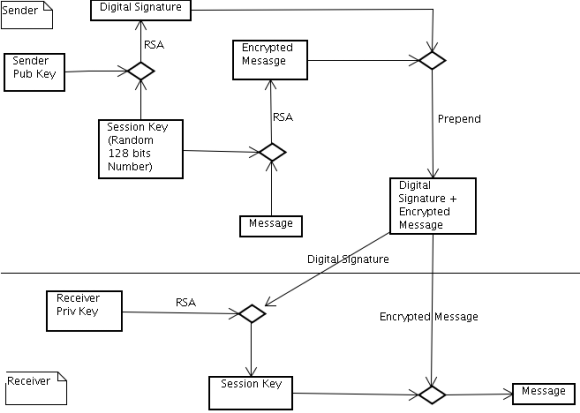
\includegraphics[scale=0.7]{images/pgp-confidentiality.png}
	\captionof{figure}{Confidencialidade em PGP}
	\label{fig:pgp-confidentiality}
\end{center}


